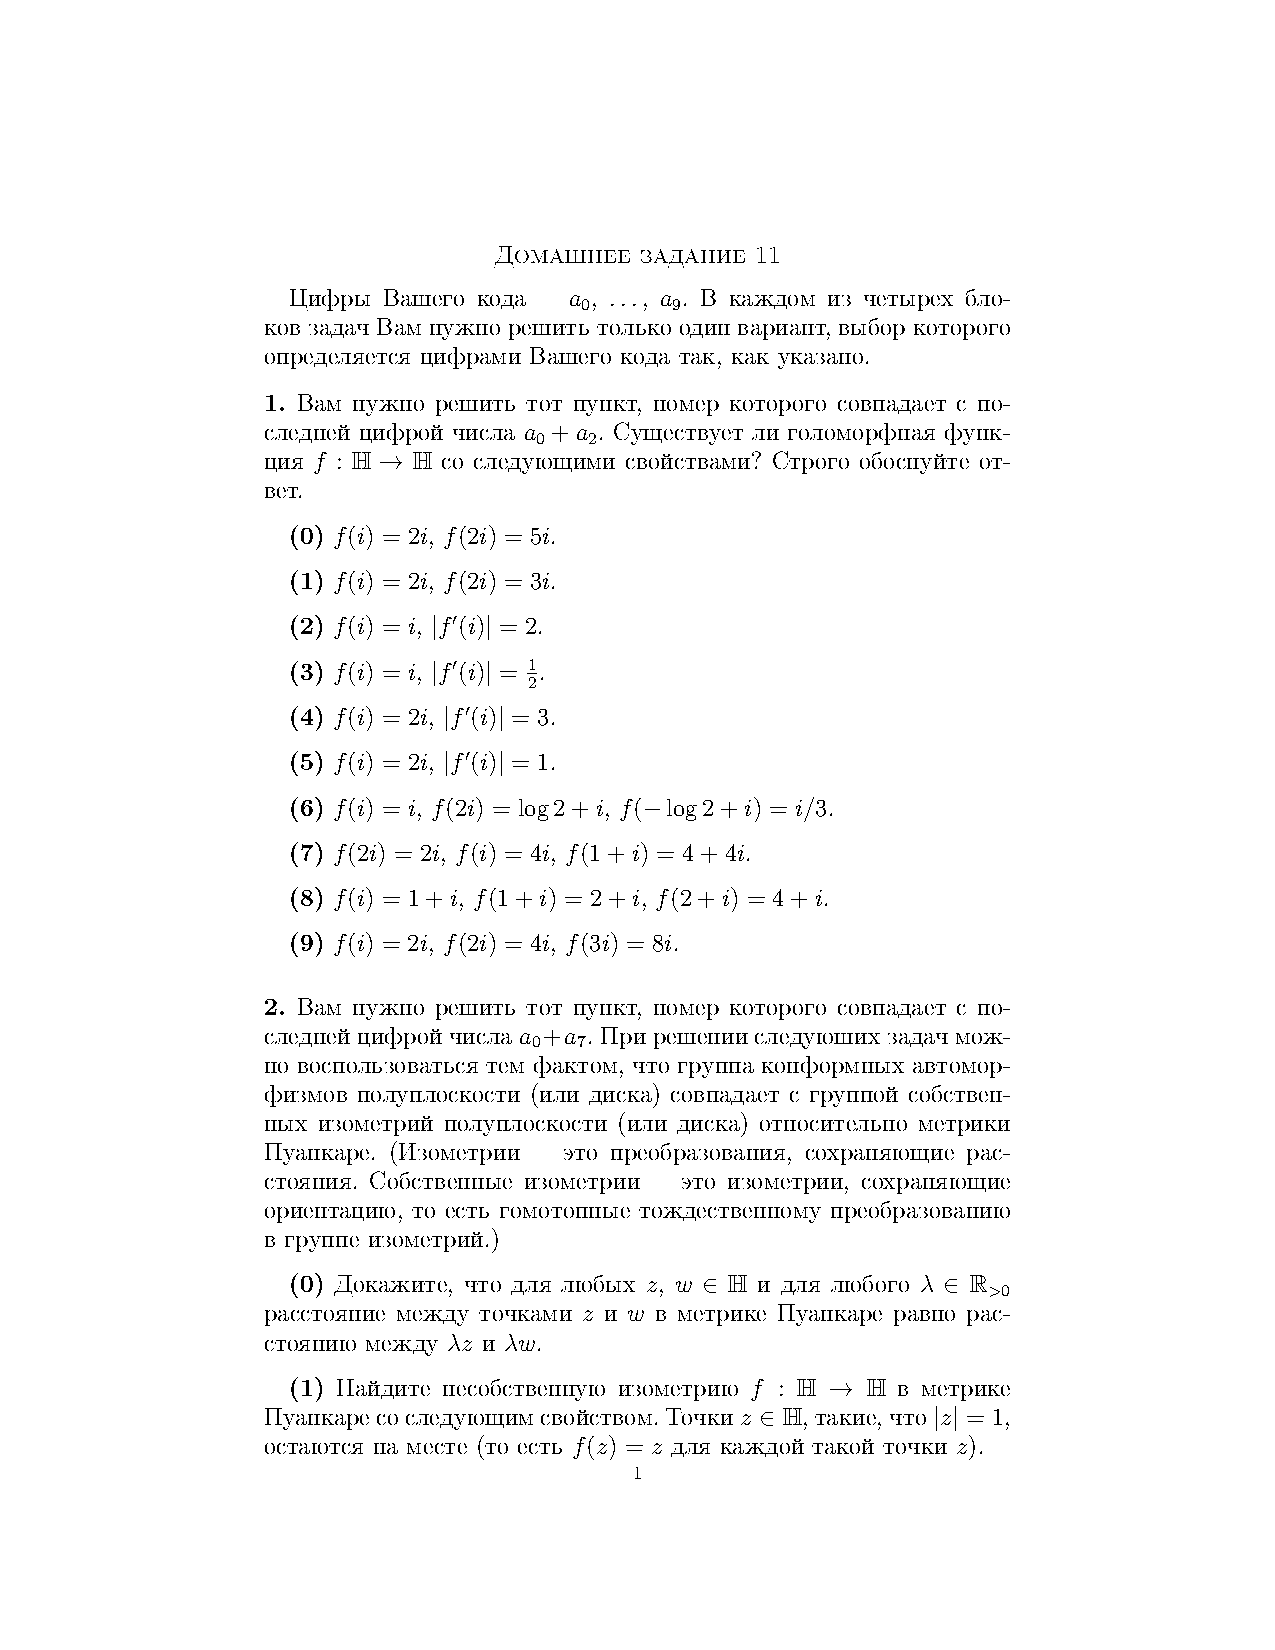
\includepdf[scale=1,pages=1-4]{Tasks/hw11}
\newpage
\section*{Решения}
\subsection*{Задача 1}
	Необходимо решить задачу $a_0 + a_2 = 1 + 8 = 9 \mod 10$\\
	Да, существует, вот пример:
	\begin{gather*}
		f(x + iy) = (2xy-x) + i(y^2-y+2+x^2)\\
		-\frac{\partial (y^2-y+2-x^2)}{\partial x} = 2x = \frac{\partial (2xy-x)}{\partial y}\\
		\frac{\partial (2xy-x)}{\partial x} = 2y-1 = \frac{\partial (y^2-y+2-x^2)}{\partial y}
	\end{gather*}
\vskip 0.4in

\subsection*{Задача 2}
	Необходимо решить задачу $a_0 + a_7 = 1 + 3 = 4 \mod 10$\\
	$C = \{z \in \mathbb{H}|\ |z|=1\}$ -- полуокружность с центром в $0$ и $R = 1$ то есть имеются 2 точки на абсолюте. Следовательно параболический автоморфизм не подходит, так как он сохраняет лишь одну точку на абсолюте.\\
	Эллиптический автоморфизм: рассмотрим автоморфизм, сохраняющий пучок прямых через $0$. Такой автоморфизм сохраняет окружности с центром в этой точке, а следовательно $f(1+i) \in A = \{|z| = \sqrt{2}\}$
	Гиперболический авторморфизм: $2$ неподвижные точки на абсолюте - это $\pm i$, тогда множество точек вида $f(1+i)$ -- эквидистанта, проходящая через $\pm i, 1+i$, то есть $\left\{z \in \mathbb{H}|\ \left|z - \frac{1}{2}\right| = \frac{\sqrt{5}}{2}\right\}$
\vskip 0.4in

\subsection*{Задача 3}
	Необходимо решить задачу $a_6 + a_9 = 9 + 6 = 5 \mod 10$\\
	Покажем, что требуемое утверждение неверно\\
	Пусть
	\begin{equation*}
		f: \overline{U} \to \mathbb{C}:
		\begin{cases}

		\end{cases}
	\end{equation*}

\vskip 0.4in

\subsection*{Задача 4}
	Необходимо решить задачу $a_0 + a_6 = 1 + 9 = 0 \mod 10$\\
	$\int\limits_{-1}^{1} \frac{dx}{\sqrt{1-x^2}} = \int\limits_{-1}^{1} \frac{dx}{\sqrt{(1-x)(1+x)}}$ -- не определено только в $1-x^2 = 0$, то есть $\pm 1$. Заметим что $f$ аналитична в $\{x \in \mathbb{C}|\ \Im{x} \geqslant 0\}$, кроме конечного числа точек, а следовательно по лемме Жордана
	\begin{equation*}
		\int\limits_{-1}^{1} \frac{dx}{\sqrt{1-x^2}}
		= \int\limits_{\gamma} \frac{dx}{\sqrt{(1-x)(1+x)}}
		= 2 \pi i (\operatorname{Res}_{1} f(x) + \operatorname{Res}_{-1} f(x))
		= 2 \pi i (\frac{1}{2i})
		= \pi
	\end{equation*}